%\documentclass[runningheads]{llncs}
%In general this is written like a lab report...need to write a technical paper. 
\documentclass[]{llncs} % "you can ignore this hint if your document works"
\usepackage{makeidx}
\usepackage{graphicx}
\usepackage{makecell}
\begin{document}
\addtocmark{Southern Methodist University} % additional mark in the TOC

\title{Laboratory Earthquake Prediction}
%\subtitle{Optional Subtitle Goes Here}

\author{Olha Tanyuk, Daniel Davieau, Charles South \and Daniel W. Engels}

%Email:  Add author emails.

\institute{Southern Methodist University, Dallas TX 75205, USA}

\maketitle

\begin{abstract}
In this paper we present a method for predicting the timing of laboratory earthquakes using machine learning. If a similar approach can be applied to improve natural earthquake prediction it will save lives. We use data collected from a laboratory experiment which exhibits similar behavior to natural earthquakes. We train a machine learning algorithm using half of the data, then predict using the other half. We compare predicted versus actual timings to measure the algorithm's accuracy. The result shows that the timing of laboratory earthquakes can be predicted up to 16 seconds in advance with 71\% accuracy. The method and result demonstrates that machine learning can help if it can be scaled from the laboratory experiment to natural earthquakes. \par
\end{abstract}

\section{Introduction}

Earthquakes cause mass destruction and loss of life. Traditional earthquake prediction methods have relied on recurrence interval based models. Because the recurrences are not constant predictions can only be made within decade spanning time windows. One such model predicted that a magnitude 6 earthquake would occur between 1985 and 1993 in the Parkfield California area but no significant event occurred until 2004 \cite{Jackson}. \par

Researchers imitate natural earthquakes in the laboratory by placing rocky material between steel blocks and applying shear stress to induce slipping. Recent improvements in the instruments \cite{Bertrand} used to measure signals have enabled the collection of larger volume data from more realistic and unpredictable laboratory earthquakes. However processing the data and detecting patterns in it has become more difficult to work with. In this paper we demonstrate that machine learning can be used to detect patterns and make predictions from realistic, unpredictable laboratory earthquake data \cite{kaggle}.\par

We use data which was collected by the Los Alamos National Laboratory and provided to the public via a Kaggle competition \cite{kaggle}. It consists of 629 million acoustic signal observations and an accompanying record of the time remaining until a laboratory earthquake (failure) occurred \cite{Bertrand}. We calculate additional statistical measures such as variance, kurtosis and skew for each observation. We use half of the data to train a machine learning algorithm. With the remaining half of the data, using only the acoustic signal as input we calculate a prediction of the time remaining until failure. We measure  accuracy by comparing the predicted to actual remaining time to failure from the original data. \par

The result shows that the timing of laboratory earthquakes can be predicted up to 16 seconds in advance with 71 percent accuracy.\par

%Conclusion
The data, hardware and software allows us to predict impending earthquakes. However we only know 8-16 seconds before failure. Therefore practical applications may be limited. This may prove useful but only applies to laboratory experiments. This could be used in industry perhaps in researching materials for wallboard, machine parts and others.\par


\section{Background}
In 2017 Los Alamos National Laboratory (LANL) researchers discovered a way to successfully predict Slow Slip Earthquakes (SSE) in a laboratory experiment that simulates natural conditions. The team trained a computer to pinpoint and analyze quasi‐periodic seismic and acoustic signals emitted during the movements along the fault. They processed massive amounts of data and identified a particular sound pattern previously thought to be noise that precedes an earthquake. The team was able to characterize the time remaining before a laboratory earthquake at all times, using time window of 1.8 sec of the data to make each prediction, with 89\% coefficient of determination \cite{LANLNews}. This result they achieved using machine learning technique Random Forest Regression. Their results were achieved using quasi‐periodic data and can not be generalized over aperiodic data. \par

In the lab, the team imitated a real earthquake using steel blocks interacting with rocky material (fault gouge) to induce slipping that emitted seismic sounds. An accelerometer recorded the acoustic emission emanating from the sheared layers \cite{LANLNews}. For the first time, researchers discovered a pattern that accurately predicted when a quake would occur. The team acknowledges that the physical traits of the lab experiment (such as shear stresses and thermal properties) differ from the real world but the application of the analysis to real earthquakes to validate their results is ongoing. This method can also be applied outside of seismology to support materials’ failure research in many fields such as aerospace and energy \cite{LANLNews}. The team’s lab results reveal that the fault does not fail randomly but in a predictable manner. The observations also demonstrate that the fault’s critical stress state, which indicates when it might slip, can be determined using exclusively an equation of state \cite{LANLNews}. So far seismologists and Earth scientists have mostly relied on catalogues of historical data to try to characterize the state of faults. These catalogs contain a minute fraction of seismic data, and remaining seismic data is discarded during analysis as useless noise. The authors discovered that—in the case of their laboratory faults--hidden in this noiselike data there are signals emitted by the fault that inform them of the state of the fault much more precisely than catalogues \cite{LANLNews}. \par

\begin{figure}[h!]
	\centering
	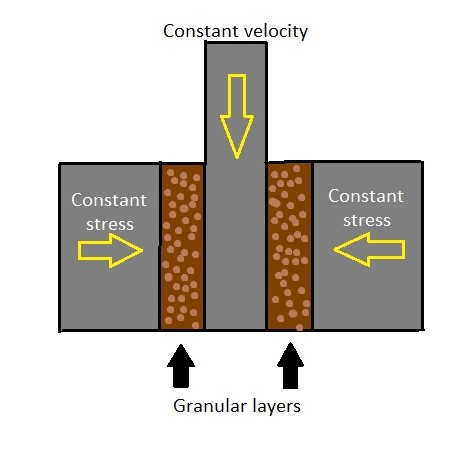
\includegraphics[width=.9\linewidth]{lab}
	\caption{}
	\label{fig:lab}
\end{figure}

The laboratory system is a two‐fault configuration that contains fault gouge material submitted to double direct shear \cite{kaggle}.
%missing image
Two fault gouge layers are sheared simultaneously while subjected to a constant normal load and a prescribed shear velocity \cite{kaggle}. The laboratory faults fail in repetitive cycles of stick and slip that is meant to mimic the cycle of loading and failure on tectonic faults \cite{kaggle}. While the experiment is considerably simpler than a fault in Earth, it shares many physical characteristics \cite{kaggle}. \par

The driving piston displaces at a very constant velocity during the inter-event time and accelerates briefly during slip \cite{Bertrand}. An accelerometer records the acoustic emission emanating from the shearing layers \cite{Bertrand}. The steel blocks are extremely stiff, so the deformation takes place largely in the gouge \cite{Bertrand}. Under a broad range of load and shear velocity conditions, the apparatus stick‐slips quasi‐periodically for hundreds of stress cycles during a single experiment and in general follows predictions from rate and state friction \cite{Bertrand}. The rate of impulsive precursors accelerates as failure approaches, suggesting that upcoming laboratory earthquake timing could be predicted \cite{Bertrand}. \par

Experimental data has 16 earthquakes. The shortest time to failure is 1.5 seconds for the first earthquake and 7 seconds for the 7th, while the longest is around 16 seconds. \par

The Extra-Trees algorithm builds an ensemble of unpruned regression trees according to the classical top-down procedure. Its two main differences with other treebased ensemble methods are that it splits nodes by choosing cut-points fully at random and that it uses the whole learning sample (rather than a bootstrap replica) to grow the trees \cite{ExtremeRandomTrees}. \par

The Extra-Trees splitting procedure uses two parameters: K (the number of attributes randomly selected at each node) and nmin (the minimum sample size for splitting a node). It is used several times with the (full) original learning sample to generate an ensemble model (we denote by M the number of trees of this ensemble) \cite{ExtremeRandomTrees}. 

The predictions of the trees are aggregated to yield the final prediction, by majority vote in classification problems and arithmetic average in regression problems \cite{ExtremeRandomTrees}. From the bias-variance point of view, the rationale behind the Extra-Trees method is that the explicit randomization of the cut-point and attribute combined with ensemble averaging should be able to reduce variance more strongly than the weaker randomization schemes used by other methods \cite{ExtremeRandomTrees}. The usage of the full original learning sample rather than bootstrap replicas is motivated in order to minimize bias \cite{ExtremeRandomTrees}. From a computational point of view, given the simplicity of the node splitting procedure we expect the constant factor to be much smaller than in other ensemble based methods which locally optimize cut-points \cite{ExtremeRandomTrees}. The parameters K, nmin and M have different effects: K determines the strength of the attribute selection process, nmin the strength of averaging output noise, and M the strength of the variance reduction of the ensemble model aggregation. These parameters could be adapted to the problem specifics in a manual or an automatic way (e.g. by cross-validation) \cite{ExtremeRandomTrees}. \par

The sklearn.ensemble module in Python programing language includes averaging algorithm based on randomized decision trees: Extra-Trees method. \par

\section{Data} 
The data used in this work is a  157.275 second chunk of seismic data (ordered in time), which is recorded at 4MHz, hence 629,145,480 data points accompanied by the time remaining until the following lab earthquake, in seconds. \par
The seismic data is recorded using a piezoceramic sensor, which outputs a voltage upon deformation by incoming seismic waves (henceforth we will use the term acoustic signal). The seismic data, which serves as the input to our analysis, is this recorded voltage, in integers. \par
% to prevent images from floating all over the place in the document: https://tex.stackexchange.com/questions/16207/image-from-includegraphics-showing-up-in-wrong-location
\begin{table}[h!]
	\begin{center}
		\caption{Data Definitions}
		\label{tab:DataDefinitions}
		\begin{tabular}{ll}
			\textbf{Acoustic Signal} & Voltage upon deformation by incoming seismic waves. \\
			\textbf{Time To Failure} & The remaining time in seconds until an actual stick-slip failure occurred.  \\
		\end{tabular}
	\end{center}
\end{table}

\begin{table}[h!]
	\begin{center}
		\caption{Sample Data}
		\label{tab:SampleData}
		\begin{tabular}{c|r} 
			\textbf{Acoustic Signal} & \textbf{Time to Failure}\\
			\hline
			12 & 1.469099998474121 \\ 
			6 & 1.469099998474121 \\ 
			8 & 1.469099998474121 \\ 
			5 & 1.469099998474121 \\ 
			8 & 1.469099998474121 \\ 
		\end{tabular}
	\end{center}
\end{table}

\begin{figure}[h!]
	\centering
	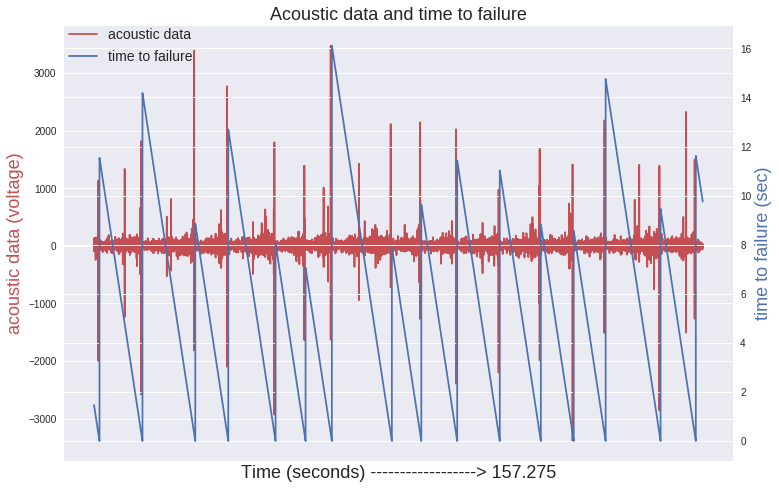
\includegraphics[width=01\linewidth]{timeSeries}
	\caption{We can see that usually acoustic data shows huge fluctuations just before the failure. Another important point: visually failures can be predicted as cases when huge fluctuations in signal are followed by small signal values.}
	\label{fig:timeseries}
\end{figure}

\begin{figure}[h!]
	\centering
	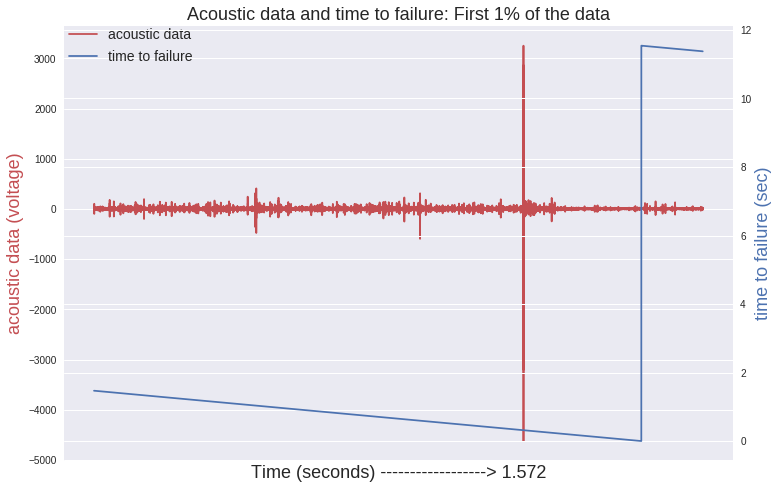
\includegraphics[width=01\linewidth]{zoomedInTimePLot}
	\caption{On zoomed-in-time plot we can see that the large oscillation before the failure is not in the last moment. There are trains of intense oscillations preceding the large one and also some oscillations with smaller peaks after it.}
	\label{fig:zoomeInTimePlot}
\end{figure}

\begin{figure}[h!]
	\centering
	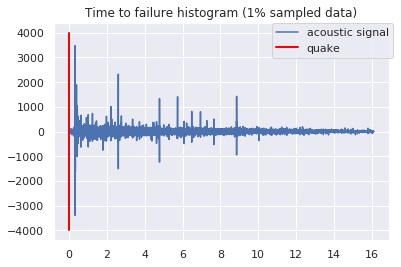
\includegraphics[width=01\linewidth]{timeToFailureHistogram}
	\caption{The voltage amplitude of acoustic precursors accelerates as failure approaches, suggesting that upcoming laboratory earthquake timing could be predicted. We used 1\% sample of the data. Red line indicates, that quake occurs, when time to failure approaches to 0. Minimum time remaining until the quake in the data is  -5.5150e+03 sec.}
	\label{fig:timeToFailureHistogram}
\end{figure}

\begin{figure}[h!]
	\centering
	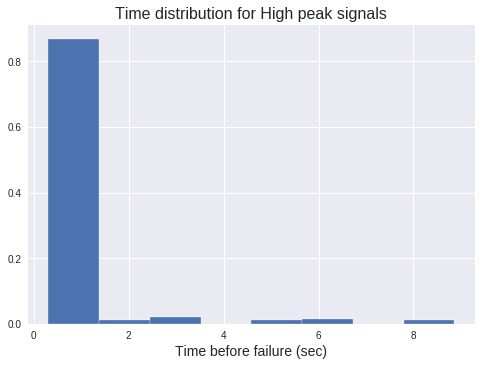
\includegraphics[width=01\linewidth]{timeDistribution}
	\caption{We found that more than 90\% of high acoustic values (absolute value greater than 1000) are around 0.31 seconds before an earthquake!}
	\label{fig:timeDistribution}
\end{figure}

\begin{figure}[h!]
	\centering
	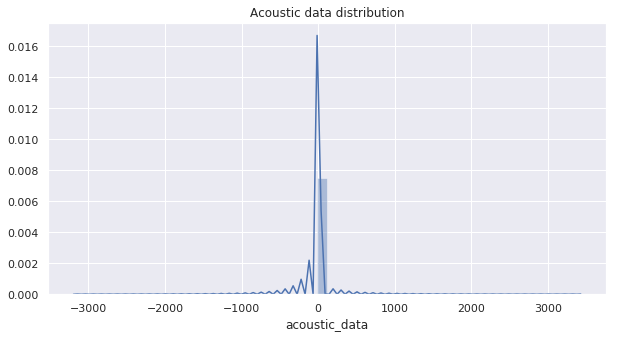
\includegraphics[width=01\linewidth]{acousticDataDistribution}
	\caption{Acoustic data distribution has a very high peak and we see outliers in both directions}
	\label{fig:acousticDataDistribution}
\end{figure}

\begin{figure}[h!]
	\centering
	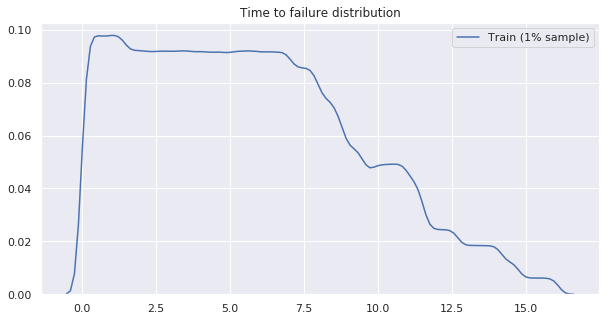
\includegraphics[width=01\linewidth]{timeToFailureDistribution}
	\caption{Distribution of time to failure seems to be right skewed. It should be normalized.}
	\label{fig:timeToFailureDistribution}
\end{figure}

\begin{figure}[h!]
	\centering
	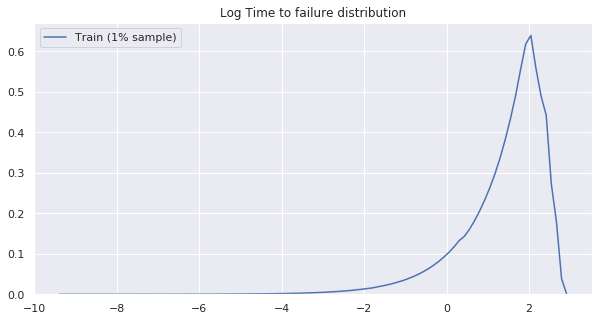
\includegraphics[width=01\linewidth]{logTimeToFailureDistribution}
	\caption{Log transformed time distribution looks more left skewed than normal.}
	\label{fig:logTimeToFailureDistribution}
\end{figure}

\begin{figure}[h!]
	\centering
	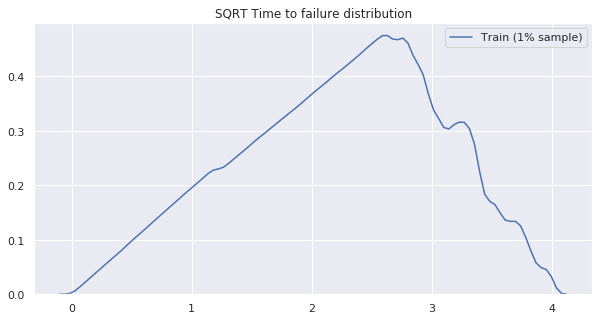
\includegraphics[width=01\linewidth]{sqrtTimeToFailureDistribution}
	\caption{The distribution of the time after square root transformation is still not ideally normal, but looks much better than the distribution of the time after log transformation.}
	\label{fig:sqrtTimeToFailureDistribution}
\end{figure}

\section{Feature Engineering}
LANL, working with quasi periodic seismic signals, achieved 0.89 coefficient of determination, using Random Forest technique and dividing data by 1.8 seconds time windows \cite{Bertrand}.  The most important features in LANL model were variance, kurtosis and threshold. We used a similar approach. Our goal is to predict the time remaining before the next failure using only moving time windows of the acoustic data. We divided our data into time windows that each contain 0.3 seconds of data (1,500,000 observations), which is small enough compared with lab quake cycle that we have (8 to 16 sec). As we discussed above, more than 90\% of high acoustic values (absolute value greater than 1000) are around 0.31 seconds before an earthquake. It makes sense to divide our data by 0.3 sec windows to reduce error at the end of the quake cycle. 

\begin{figure}[h!]
	\centering
	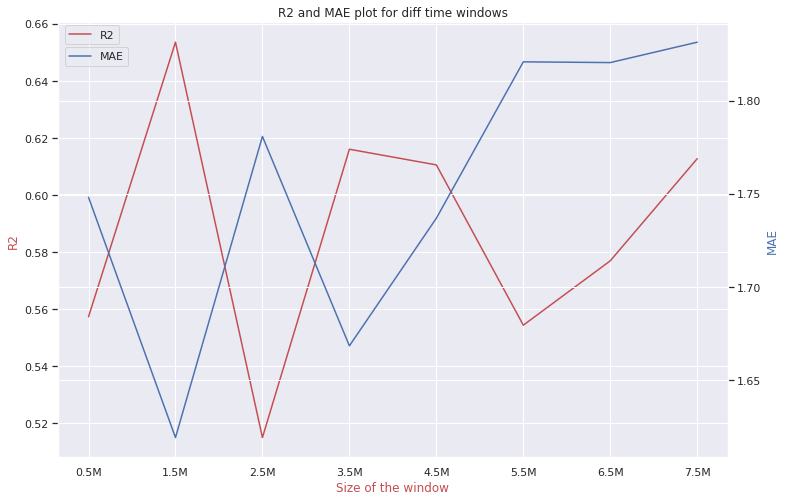
\includegraphics[width=01\linewidth]{rSquaredandMAE}
	\caption{We checked how sensitive our results are to the size of the window, and found that the highest R2 and smallest MAE we were able to get with 1.5M observations in each time window.}
	\label{fig:rSquaredandMAE}
\end{figure}

So our new data set is 419 time windows (0.3 sec long each).  From each time window, we compute a set of 95 potentially relevant statistical features (e.g., mean, variance, kurtosis, min/max, threshold and so on), but using feature importance we found that only the following were important:
\begin{table}[h!]
	\begin{center}
		\caption{Engineered Features}
		\label{tab:engineeredFeatrures}
		\begin{tabular}{l} 
Standard Deviation \\
90\% Quantile \\
95\% Quantile \\
99\% Quantile \\
Absolute Standard Deviation \\
Average Rolling Standard Deviation for 100, 1000 and 10000 observations \\
Variance of Rolling Standard Deviation for 100, 1000 and 10000 observations \\
Minimum Rolling Standard Deviation for 100, 1000 and 10000 observations \\
1\% Quantile of rolling standard deviation for 100, 1000, 10000 observations \\
5\% Quantile of rolling standard deviation for 100, 1000, 10000 observations \\
10\% Quantile of rolling standard deviation for 100, 1000, 10000 observations \\
90\% Quantile of rolling standard deviation for 100, 1000, 10000 observations \\
95\% Quantile of rolling standard deviation for 100, 1000, 10000 observations \\
99\% Quantile of rolling standard deviation for 100, 1000, 10000 observations \\
Variance of Rolling Absolute Mean for 100, 1000 and 10000 observations \\
		\end{tabular}
	\end{center}
\end{table}

We apply different machine learning techniques such as the Random Forest Regressor, XGB Regressor,  Decision Tree Regressor, LGBM Regressor, Extra Trees Regressor to the new continuous values that we got, analysing acoustic time series data. \par
In order to avoid correlation between new features we applied principal component analysis.  Instead of using 35 features, we created just 5 that represented 99.9\% of the full data variation. \par
We use a 50/50 continuous split of the full time series for use as training and testing data sets respectively. Contiguity of train and test data sets is important, since we want to minimize contamination of the training data with information about the test data. \par
We computed regularization hyper-parameters for each machine learning predicting techniques by random grid search based on a 3-fold cross-validation.

\section{Results}
We run different techniques on a training data set (50\% of the full data) before principal component analysis and after. Principal component analysis did not improve our findings significantly. We quantify the accuracy of our model using $r^2$ (the coefficient of determination) and MAE (mean absolute error), applying predicting model on test data set. The best results we achieved using  Extra Trees Regressor technique: MAE: 1.61, $r^2 = 0.65$. \par

Hyper-parameters for this technique are 'maxdepth': 25,  'maxfeatures': 'auto', 'minsamplesleaf': 16,  'minsamplessplit': 30, 'minweightfractionleaf': 0.06225661421078982,  'nestimators': 400. The Extra Trees Regressor overview is presented in the section 2.2.

\begin{figure}[h!]
	\centering
	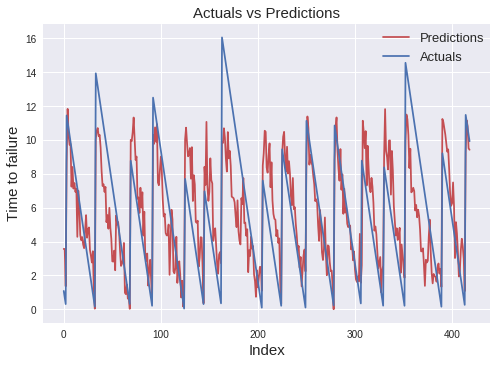
\includegraphics[width=01\linewidth]{results1}
	\caption{When making a prediction (red curve), we emphasize that there is no past or future information considered: each prediction uses only the information within one single time window of the acoustic signal.}
	\label{fig:results1}
\end{figure}

\begin{figure}[h!]
	\centering
	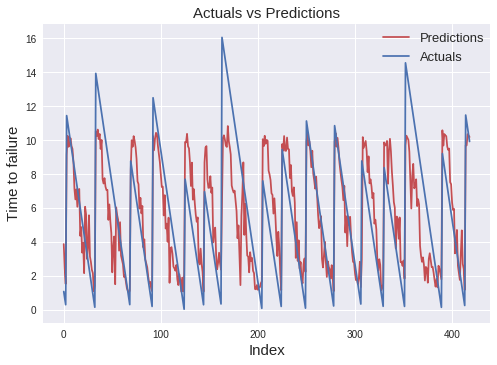
\includegraphics[width=01\linewidth]{results2}
	\caption{Results we achieved using AdaBoostRegressor: MAE: 1.67, r2score: 0.62 (Fig.11).
		Hyper-parameters for this technique are: 'learningrate': 0.018261985736355728, 'loss': 'square', nestimators = 500, baseestimator=Ridge(alpha=1).
	}
	\label{fig:results2}
\end{figure}

\section{Analysis}

The most accurate results with coefficient of determination 0.65 and mean absolute error 1.61 seconds we got using Extra Trees Regressor. The most important features are shown on Fig. 12. Top 5 are 90\% and 95\% Quartiles rolling standard deviations, standard deviation of rolling absolute mean, average rolling standard deviation.
\begin{figure}[h!]
	\centering
	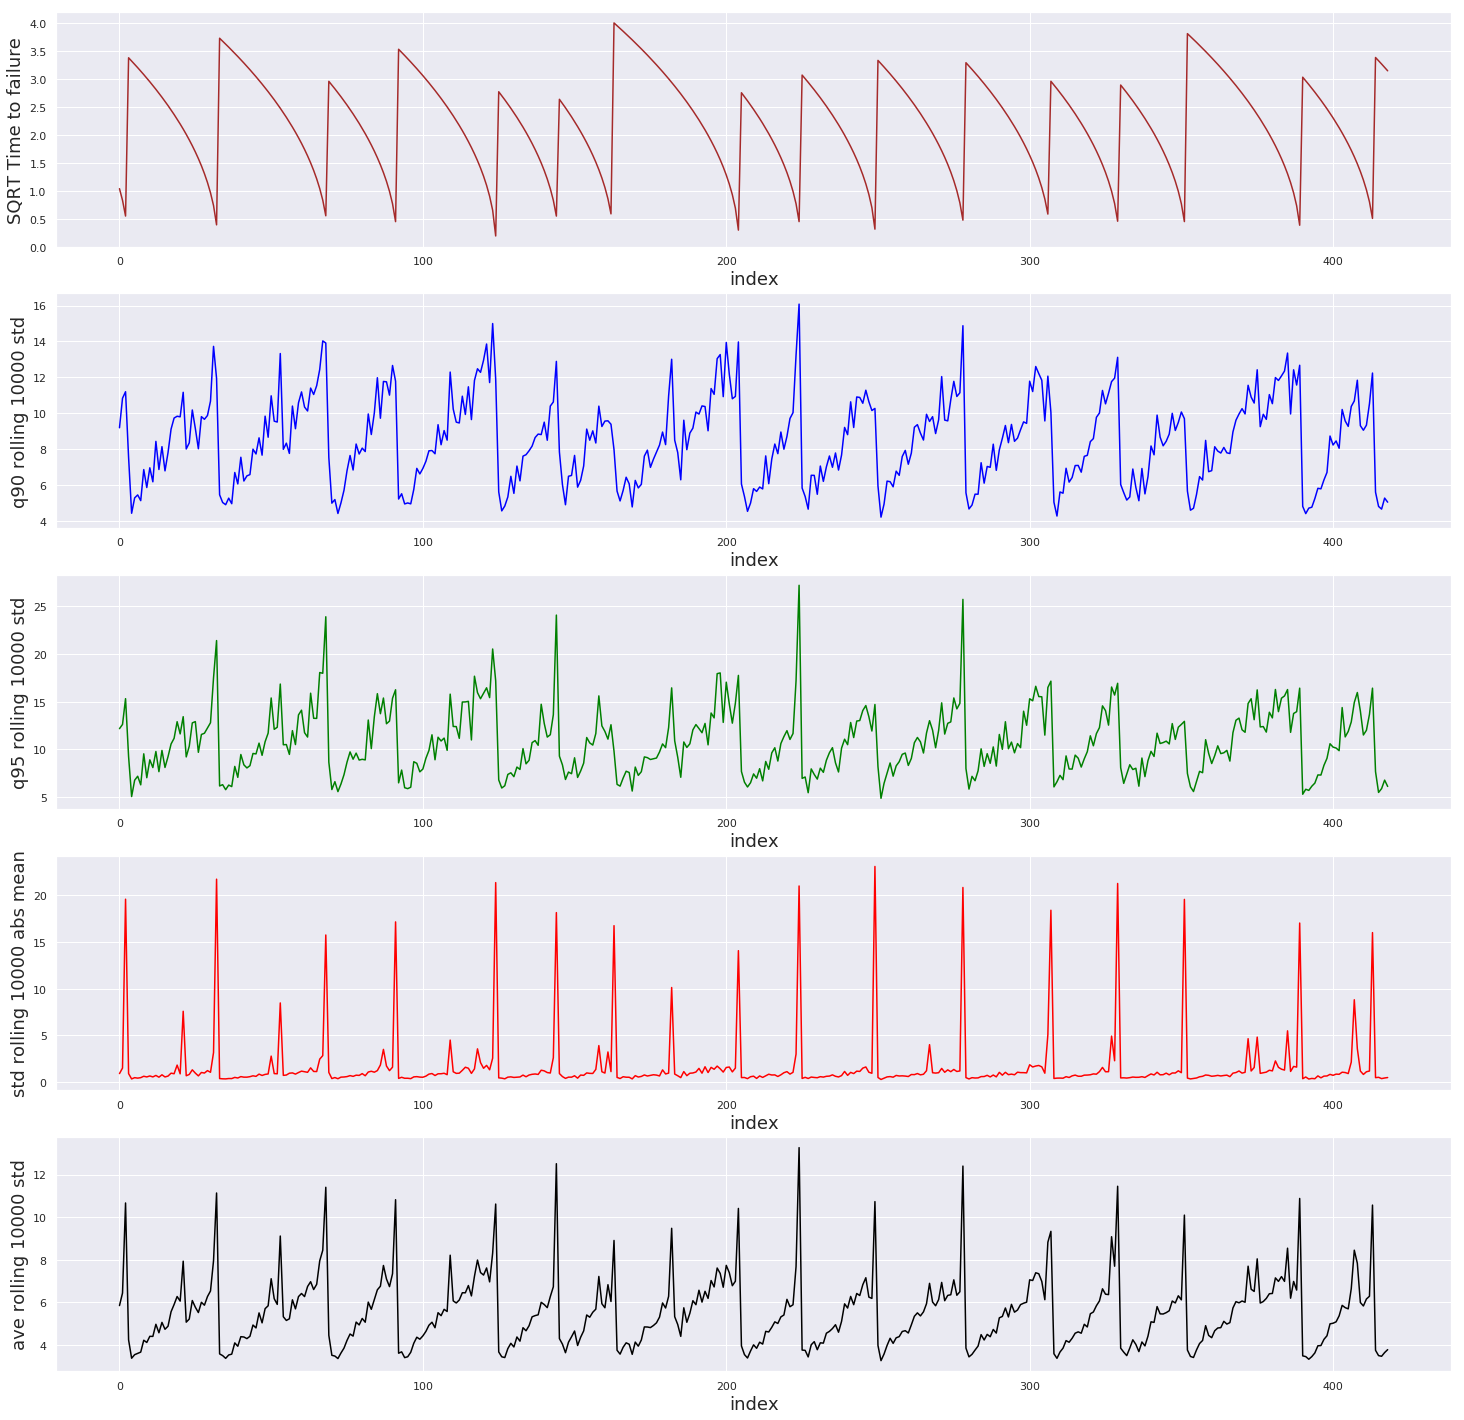
\includegraphics[width=01\linewidth]{analysis}
	\caption{}
	\label{fig:analysis}
\end{figure}


\section{Ethics}

Our responsibility to report our results has to be weighed with our responsibility not to cause social disturbance. If the method demonstrated in this paper is scaled and applied to predict natural earthquakes this balance must be considered. Unwarranted predictions could have affects on personal property value while failure to report warranted predictions could result in loss of life or avoidable property damage. \cite{Ayhan}. \par

\section{Conclusions}

The results show that laboratory earthquakes can be predicted with 71\% accuracy up to 16 seconds in advance. The acoustic signal measurement is an indicator of imminent failure. The recurrence interval is not needed to achieve the 71\% accuracy prediction. \par

In this study we are using only 157 seconds of data. Future work should introduce higher volumes of data to determine if accuracy can be improved. Also the combination of the acoustic signal and the recurrence interval should be tested to determine it's affect on accuracy. 
\par

%References
\bibliographystyle{splncs}
\bibliography{myBibliography}

\end{document}
